\chapter{Evaluation}
% \label{ch:relatedwork}
In order to evaluate the efficiency of our approach, we evaluated it on two real-world applications. These apps 
are on completely different hardware with a completely different framework and different use cases. We will 
present and discuss our results for both of them individually by first explaining the experimental setups involved 
and then provide reasoning for the results obtained. \\

\section{Experimental Setup \textemdash TempSens}
For our first experimental setup, the application we use is called \texttt{TempSens}. It is a mock app that 
was developed from scratch. It continuously monitors and log sensor data from a DHT11 sensor which is used 
to monitor temperature and humidity levels. Overall, 
the app is very simple and has a basic functionality: continuously monitor data and communicate it with the server 
every 60 seconds. The hardware configuration in this setting utilizes a Raspberry Pi 4 Model B running 
a headless Raspbian OS as an edge device where it functions as a client, and a remote server deployed on a MacBook 
Pro running Big Sur. \\
Raspberry Pi 4 Model B houses a System-on-Chip (SoC) which makes it much more affordable and reliable in terms of 
computing capability. It uses BCM2711 as its SoC type which is one of more energy and cost effective alternatives 
than its previous counterparts. The \texttt{TempSensClient} is written in Python 3 and uses RPi.GPIO to interface 
with the sensors. Figure \ref{fig:gpio} shows an extension board that is used to connect sensors to the Raspberry Pi. 
Figure \ref{fig:gpiotable} on the other hand provides the naming methods used for WiringPi, Board and the 
intrinsic pin name for GPIO extension board. For instance, for GPIO27, the WiringPi naming method is 2, Board naming 
method is 13 and its intrinsic name is GPIO2 \cite{gpio}. The overall circuitry resembles that in the figure \ref{fig:circuit}.
WiringPi \cite{wiring} is the CPP library for Raspberry Pi to interact with a GPIO extension board and Board 
\cite{pypi} is a Python library 
for the same purpose. 


\begin{figure}
    \begin{center}
        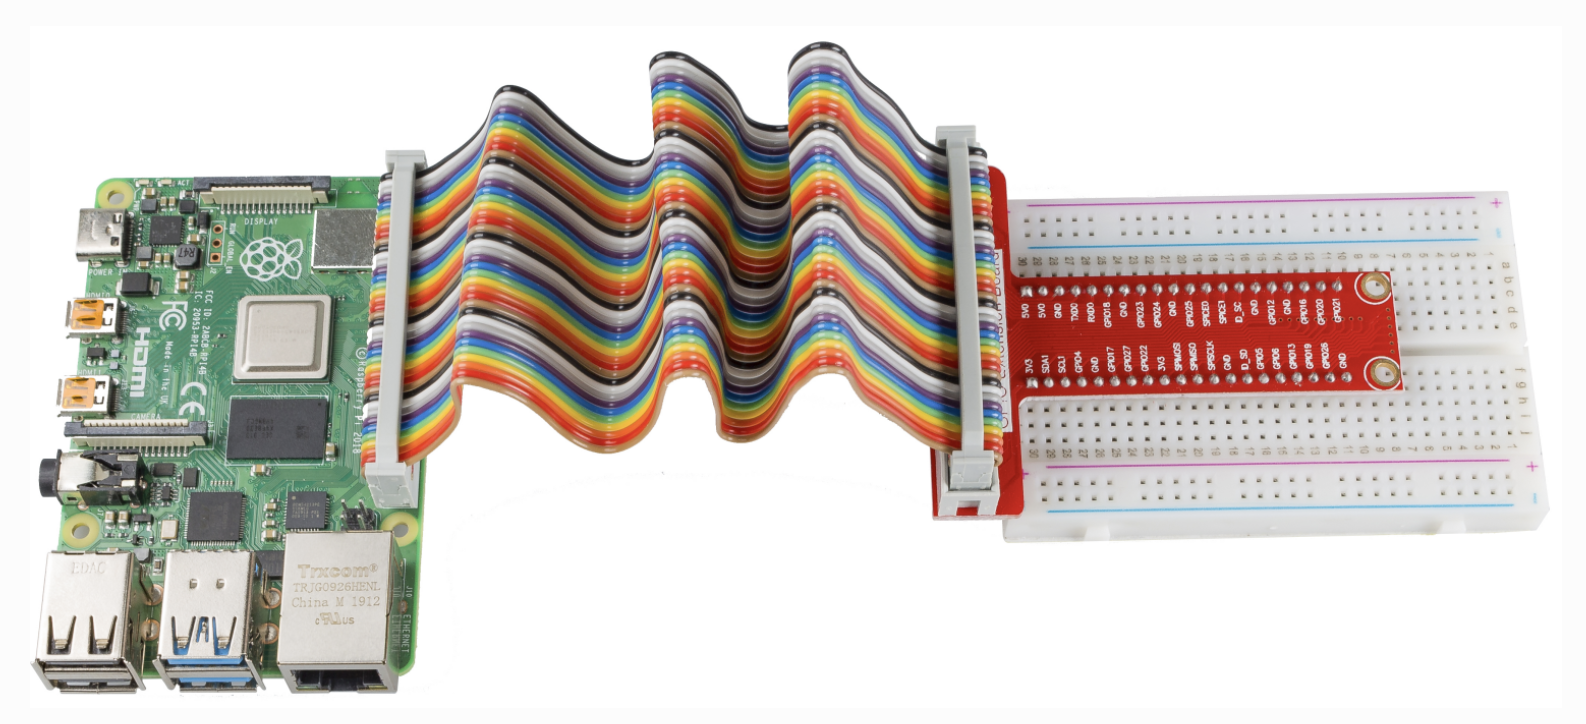
\includegraphics[scale=0.55]{Figs/gpio.png}    
    \end{center}
    \caption{A GPIO extension board \cite{gpio}}
    \label{fig:gpio}
\end{figure}

\begin{figure}
    \begin{center}
        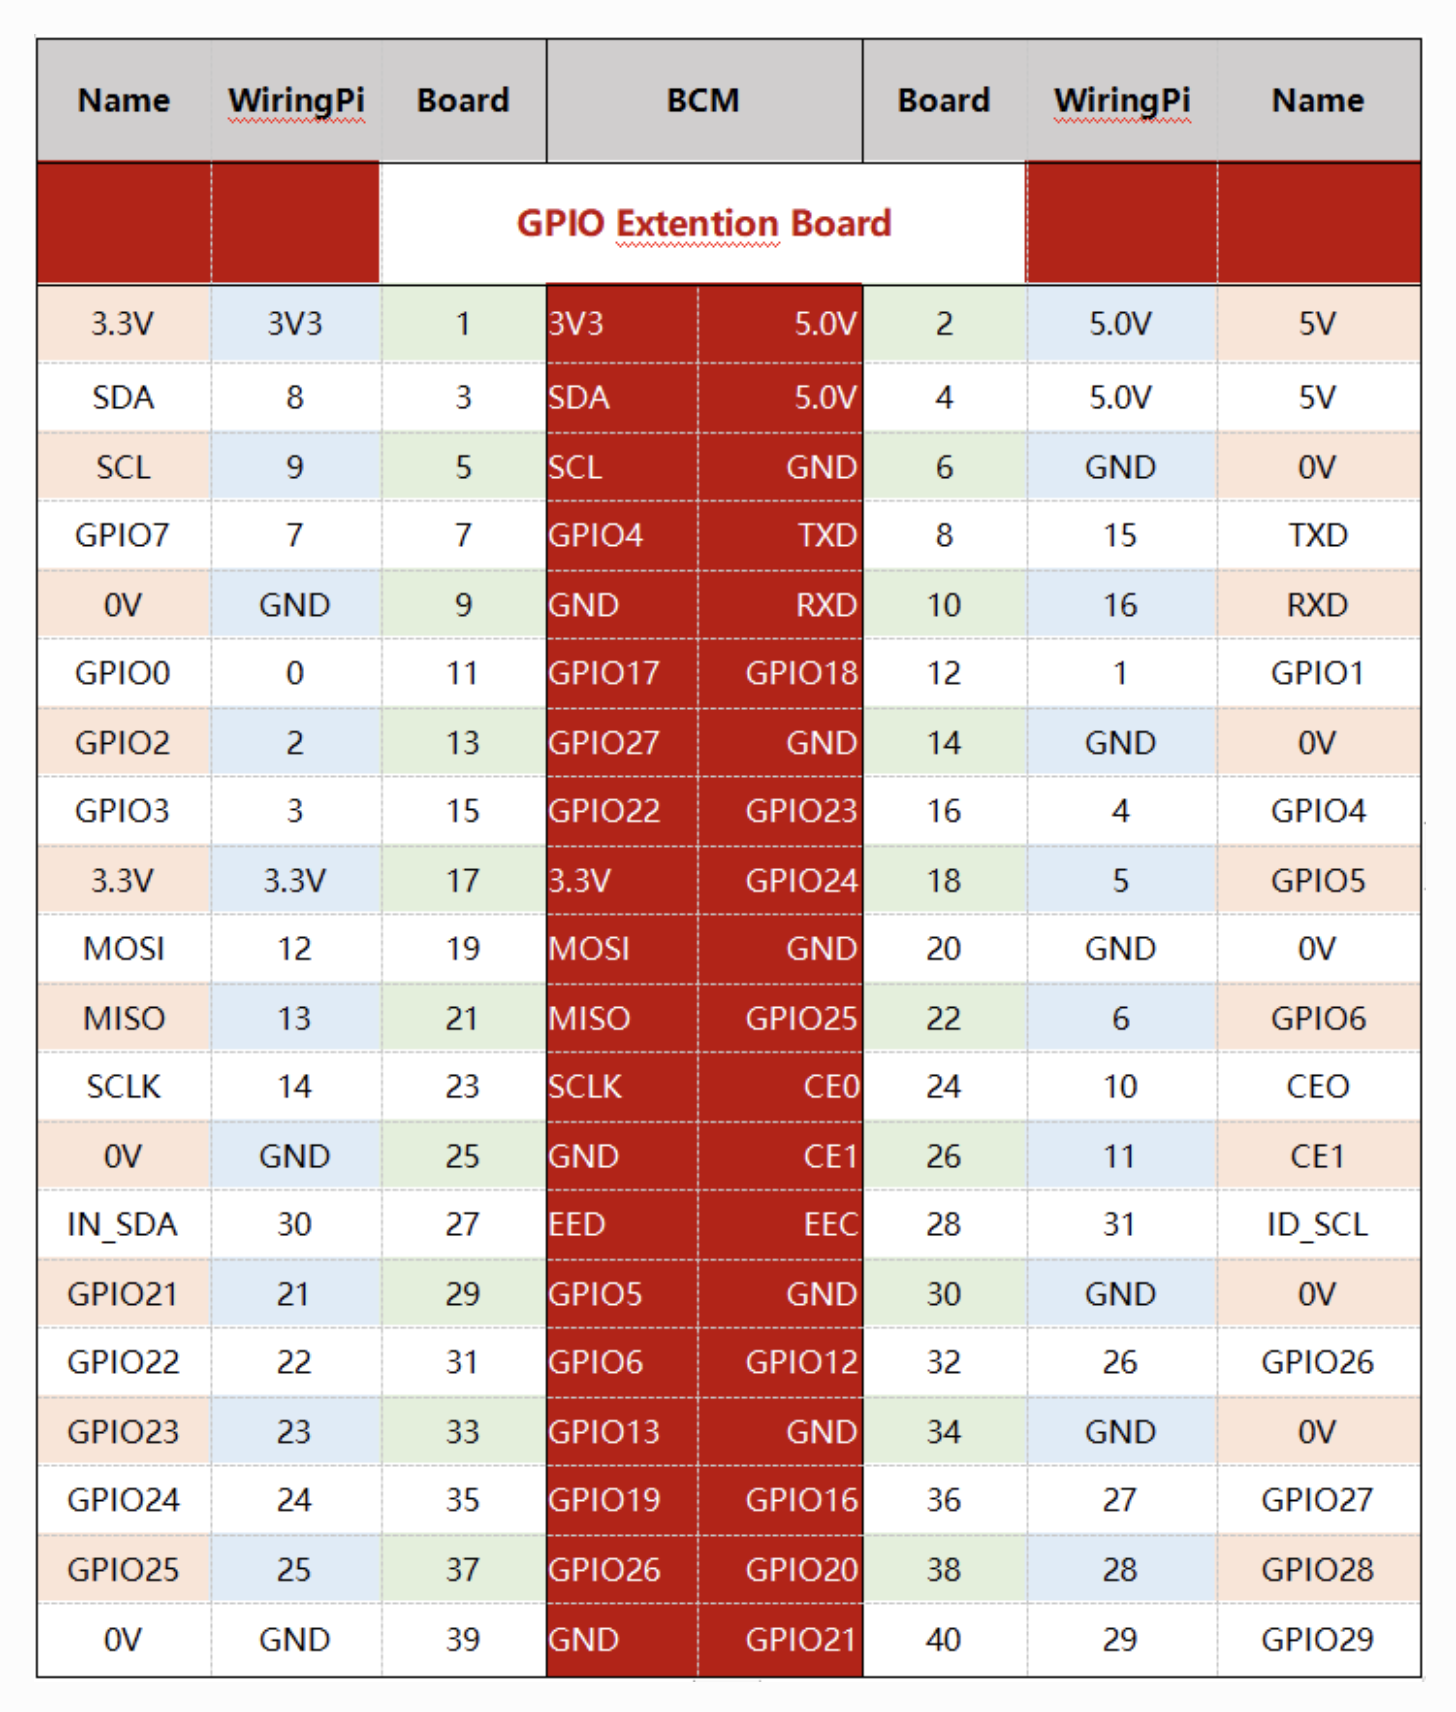
\includegraphics[scale=0.45]{Figs/gpiotable.png}    
    \end{center}
    \caption{Naming methods for WiringPi and Board \cite{gpio}}
    \label{fig:gpiotable}
\end{figure}

\begin{figure}
    \begin{center}
        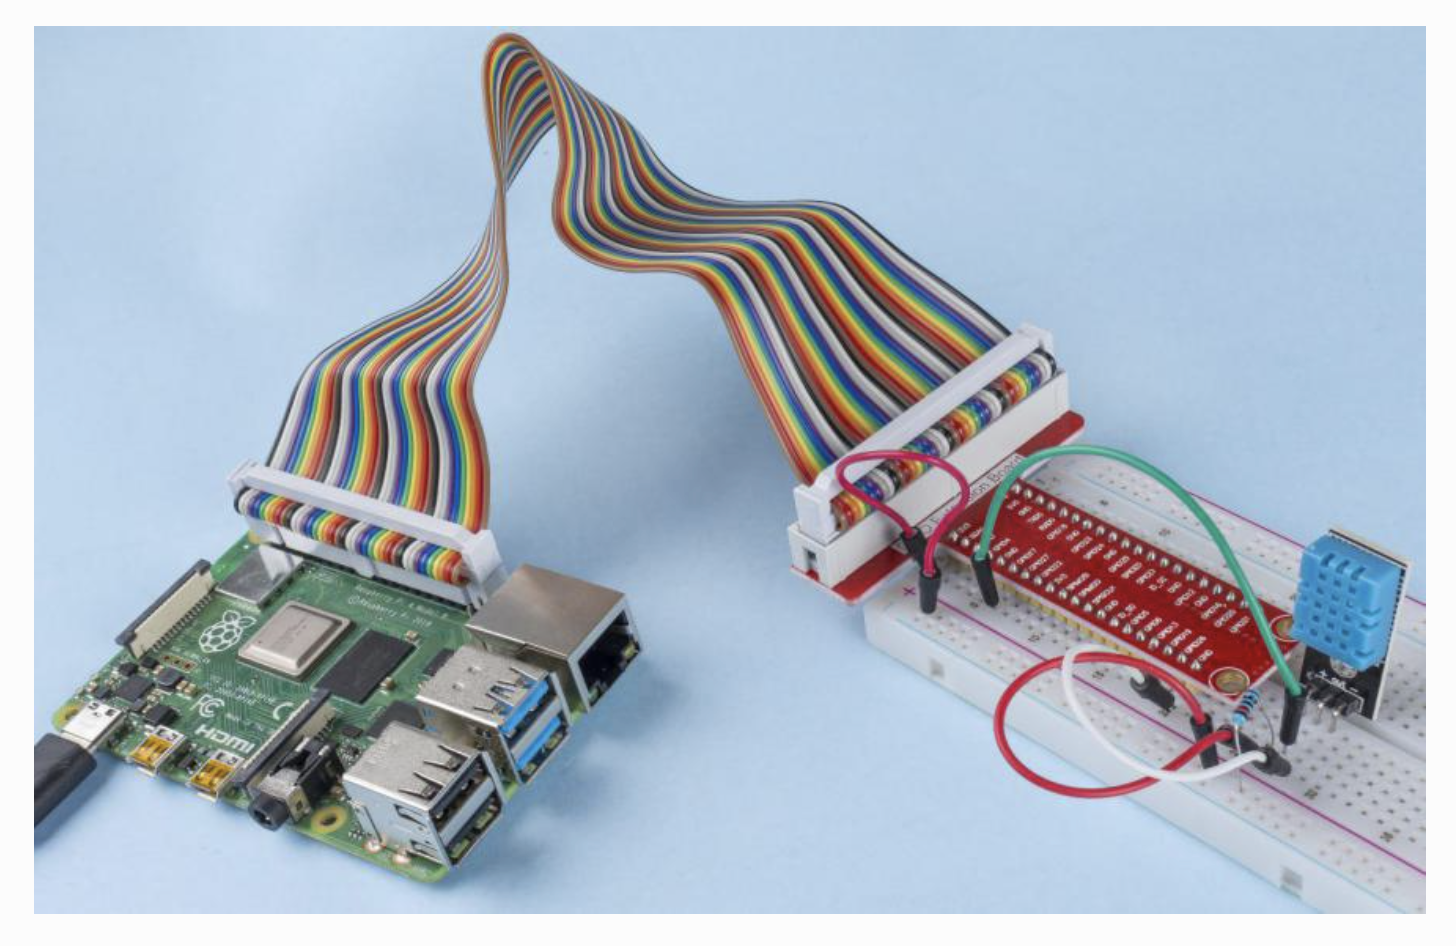
\includegraphics[scale=0.45]{Figs/circuit.png}    
    \end{center}
    \caption{TempSens Hardware Configuration  \cite{circuit}}
    \label{fig:circuit}
\end{figure}

The communication is done over TCP/IP with the help of socket programming. The \texttt{TempSensServer} 
is a bare-bone server which just displays the received information in a proper format. The client collects data for 
one minute before sending the accumulated data to the server. By default, it uses 512 bytes as chunk size. \\
Based off figure \ref{fig:bcm}, the estimated power consumption of wifi adapter is \texttt{1.542} Watts. This 
is calculated after computing the mean average sum of different power modes for different current values 
corresponding to the voltage. In order to compute the optimal chunk size, the python script to determine the 
chunk size was run on the Raspberry Pi 4. \\

\begin{figure}
    \begin{center}
        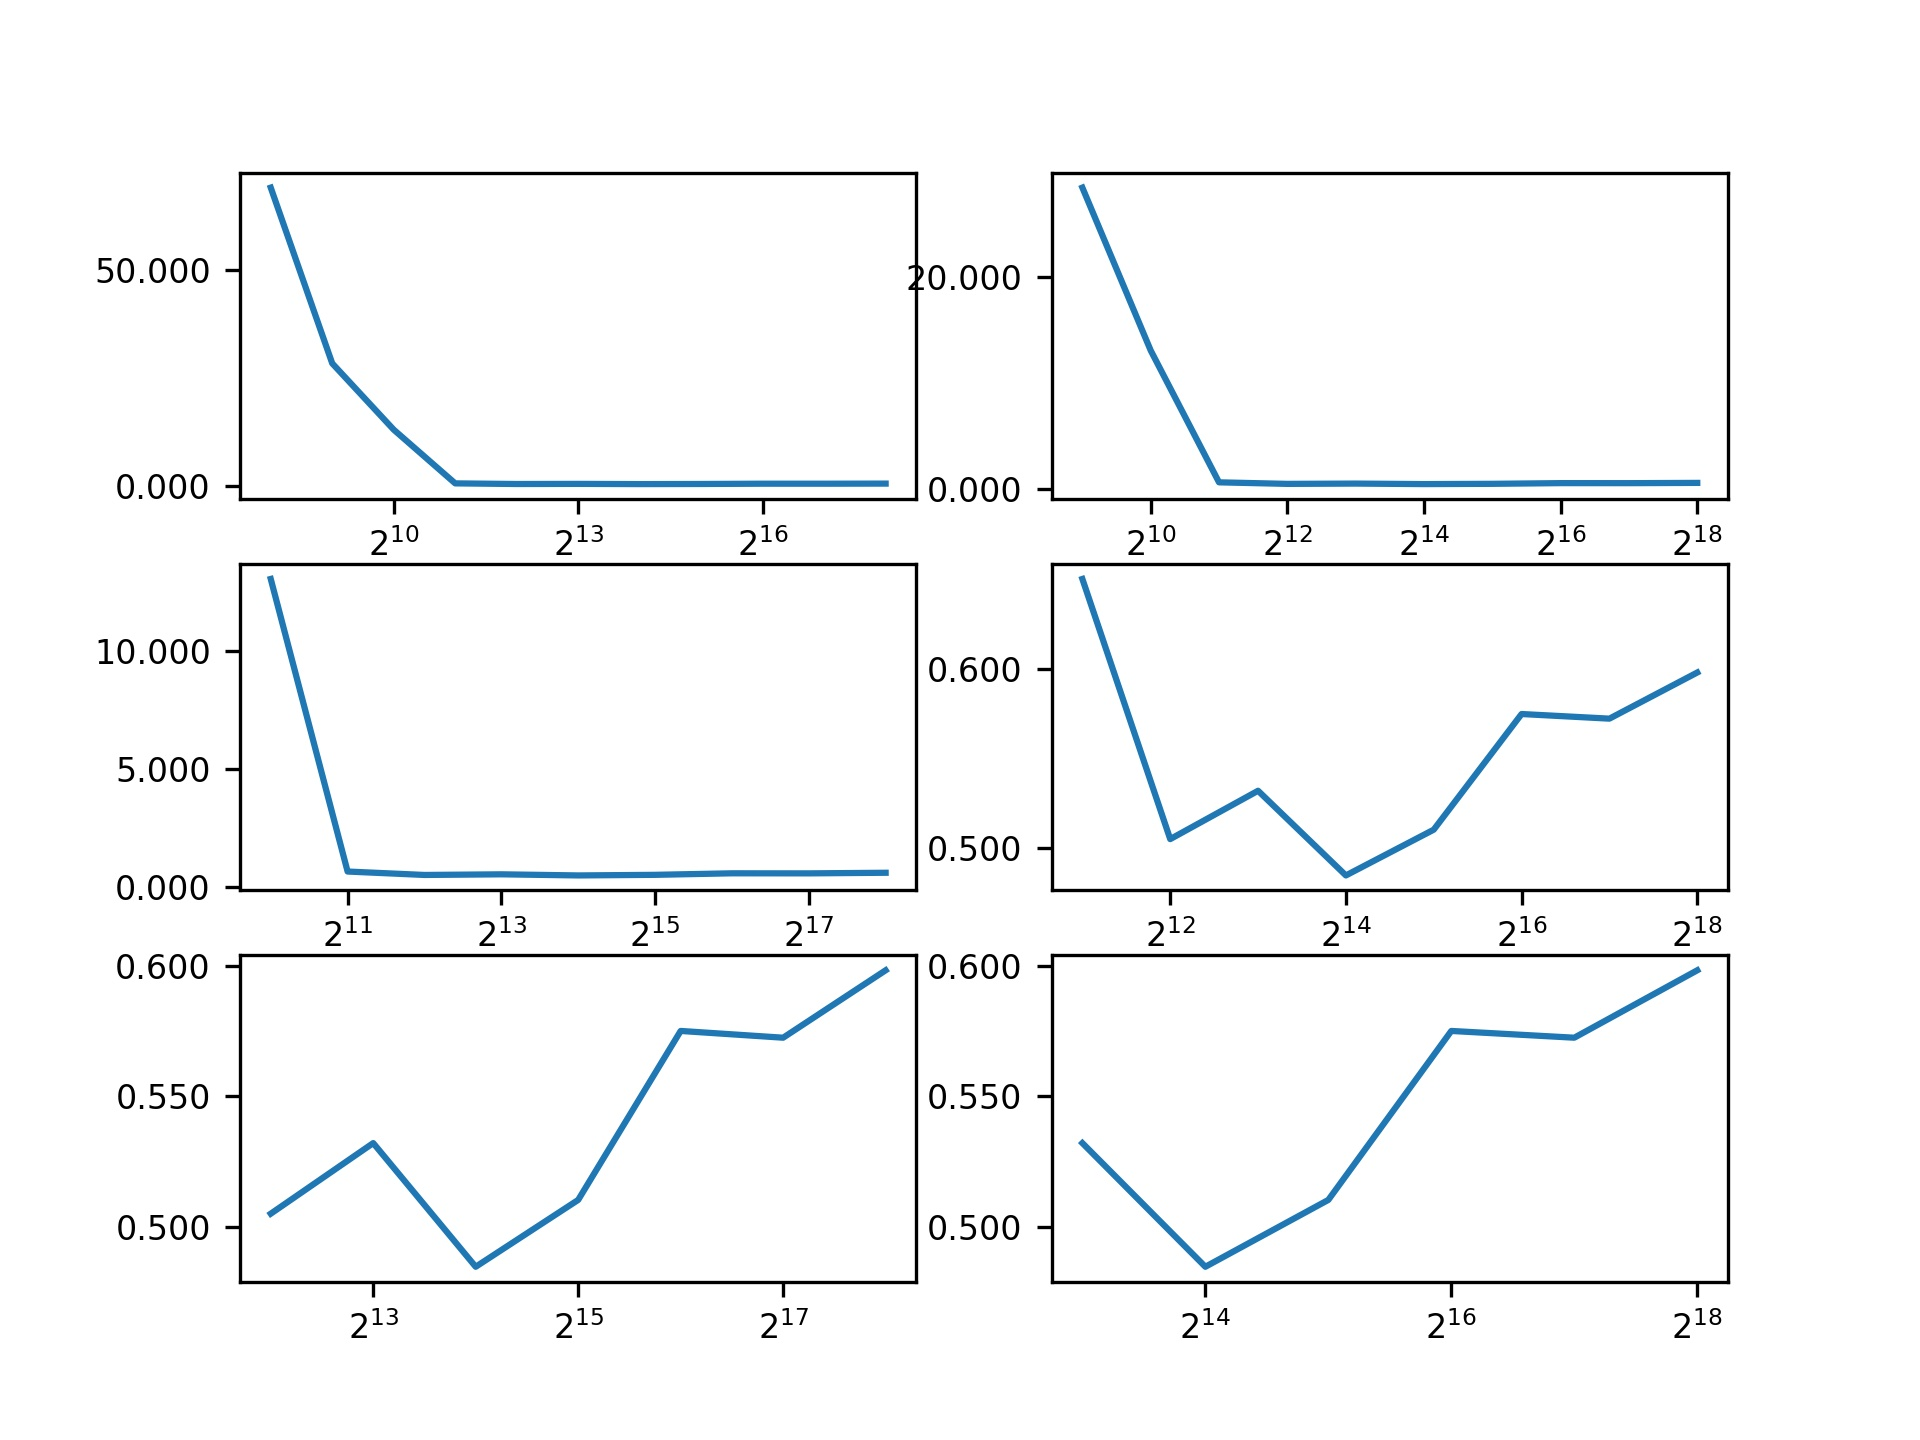
\includegraphics[scale=0.23]{Figs/epbpi.png}    
    \end{center}
    \caption{EPB for different chunk sizes (Chunk Size (x-axis) and Energy in microJ (y-axis)) - Raspberry Pi 4}
    \label{fig:epbpi}
\end{figure}

Figure \ref{fig:epbpi} shows that energy consumption does not linearly depend on chunk size. If that were the case, 
we would have got a straight line. However, what we observe is a global minima and around \texttt{$2^{14}$} on 
the x-axis, we see that's where the lowest amount of energy is being consumed per byte. This suggests that 
for the \texttt{TempSens} app to have optimal energy consumption for communication, the preferred chunk size 
should be \texttt{$2^{14}$} as it would consume the lowest amount of energy. It can also be seen that EPB at \texttt{$2^{14}$} 
is significantly lower than that at the initial value of \texttt{$2^{8}$}. Figure \ref{fig:epbpi} shows multiple 
subplots each for a different range of chunk sizes. The idea behind this is to show that even though the energy 
usage looks pretty much the same when seen in the top-left and top-right plot, but when you actually zoom in 
and see the bottom-left and bottom-right plots, you realize that the energy usage is not that linear anymore. 
There's clearly a global minima present and it will be different for different devices due to varying 
hardware and software configuration but with our work we can definitely find it. \\
Based on the values obtained from this experiment, and then replace them with the default values in \texttt{TempSensClient}, 
the total amount of time for which battery life was prolonged solely due to saving energy in communication cost 
was about 3 minutes. However, one other use-case of this approach is to be able to determine the intervals at 
which one should communicate data, if it allows. In the case of \texttt{TempSens}, its quite flexible as 
the information being communicated is not time sensitive and the use-case is not that critical. This suggests that 
an optimal interval would be just when the app collects enough amount of data (\texttt{$2^{14}$}). For this app, 
it turned out to be 120 seconds which is double the original interval break. Applying this optimization, we were 
able to prolong the battery time of one charge cycle by 7 minutes. Even though apparently it doesn't sound like much 
but keep in mind this is just with optimizing communication cost which is usually in terms of microJoules. 
Comparatively, that is a considerable improvement in the overall scheme of things. On the other hand, it would 
not have mattered much if the energy usage of the whole device was dependent on a sensor which consumes 
much more energy as compared to the wifi adapter as we will discuss it in the next experimental setup. \\

\section{Experimental Setup \textemdash Fall Detection App}
For this experiment, we test our approach on the Fall Detection App \cite{falld}. It is a real-world fall detection app 
that uses machine learning to predict whether a person wearing a smartwatch has fallen or not. Unlike the app mentioned in 
\cite{falld}, the version we test our approach on has majority of the app functionality on the smartwatch itself, whereas the 
mobile phone is just used to create and load profiles. It uses accelerometer data to predict whether a fall has occurred or not. 
It continuously logs this information and stores it in a local Couchbase database \cite{couchbase}. The app is written in 
native Java/Android for WearOS. The app works in a simple manner. First, since the app by default has a generic detection 
model, the user needs to calibrate it for themselves by wearing the app for around 3 hours. The model is then retrained with 
personalized accelerometer data for more accurate predictions. The server is maintained on a campus Mercury server \cite{mercury} which 
is not publicly accessable to keep confidential data safe. It also houses the training script to retrain the models. The app itself 
communicates data with this server using HTTP POST. The app uses OkHttp \cite{ok} as a communication API between the client and the server.\\
The smartwatch used is Huawei Watch 2 Sport Model LEO-BX9 running WearOS version 2.14. The partner app to create and load profiles 
is running on an LG Nexus 5 running Android 8.0. The Huawei Watch 2 Sport uses a Qualcomm chipset housing a WCN3620 wireless 
connectivity integrated circuit \cite{wcn3620}. \\

\begin{figure}
    \begin{center}
        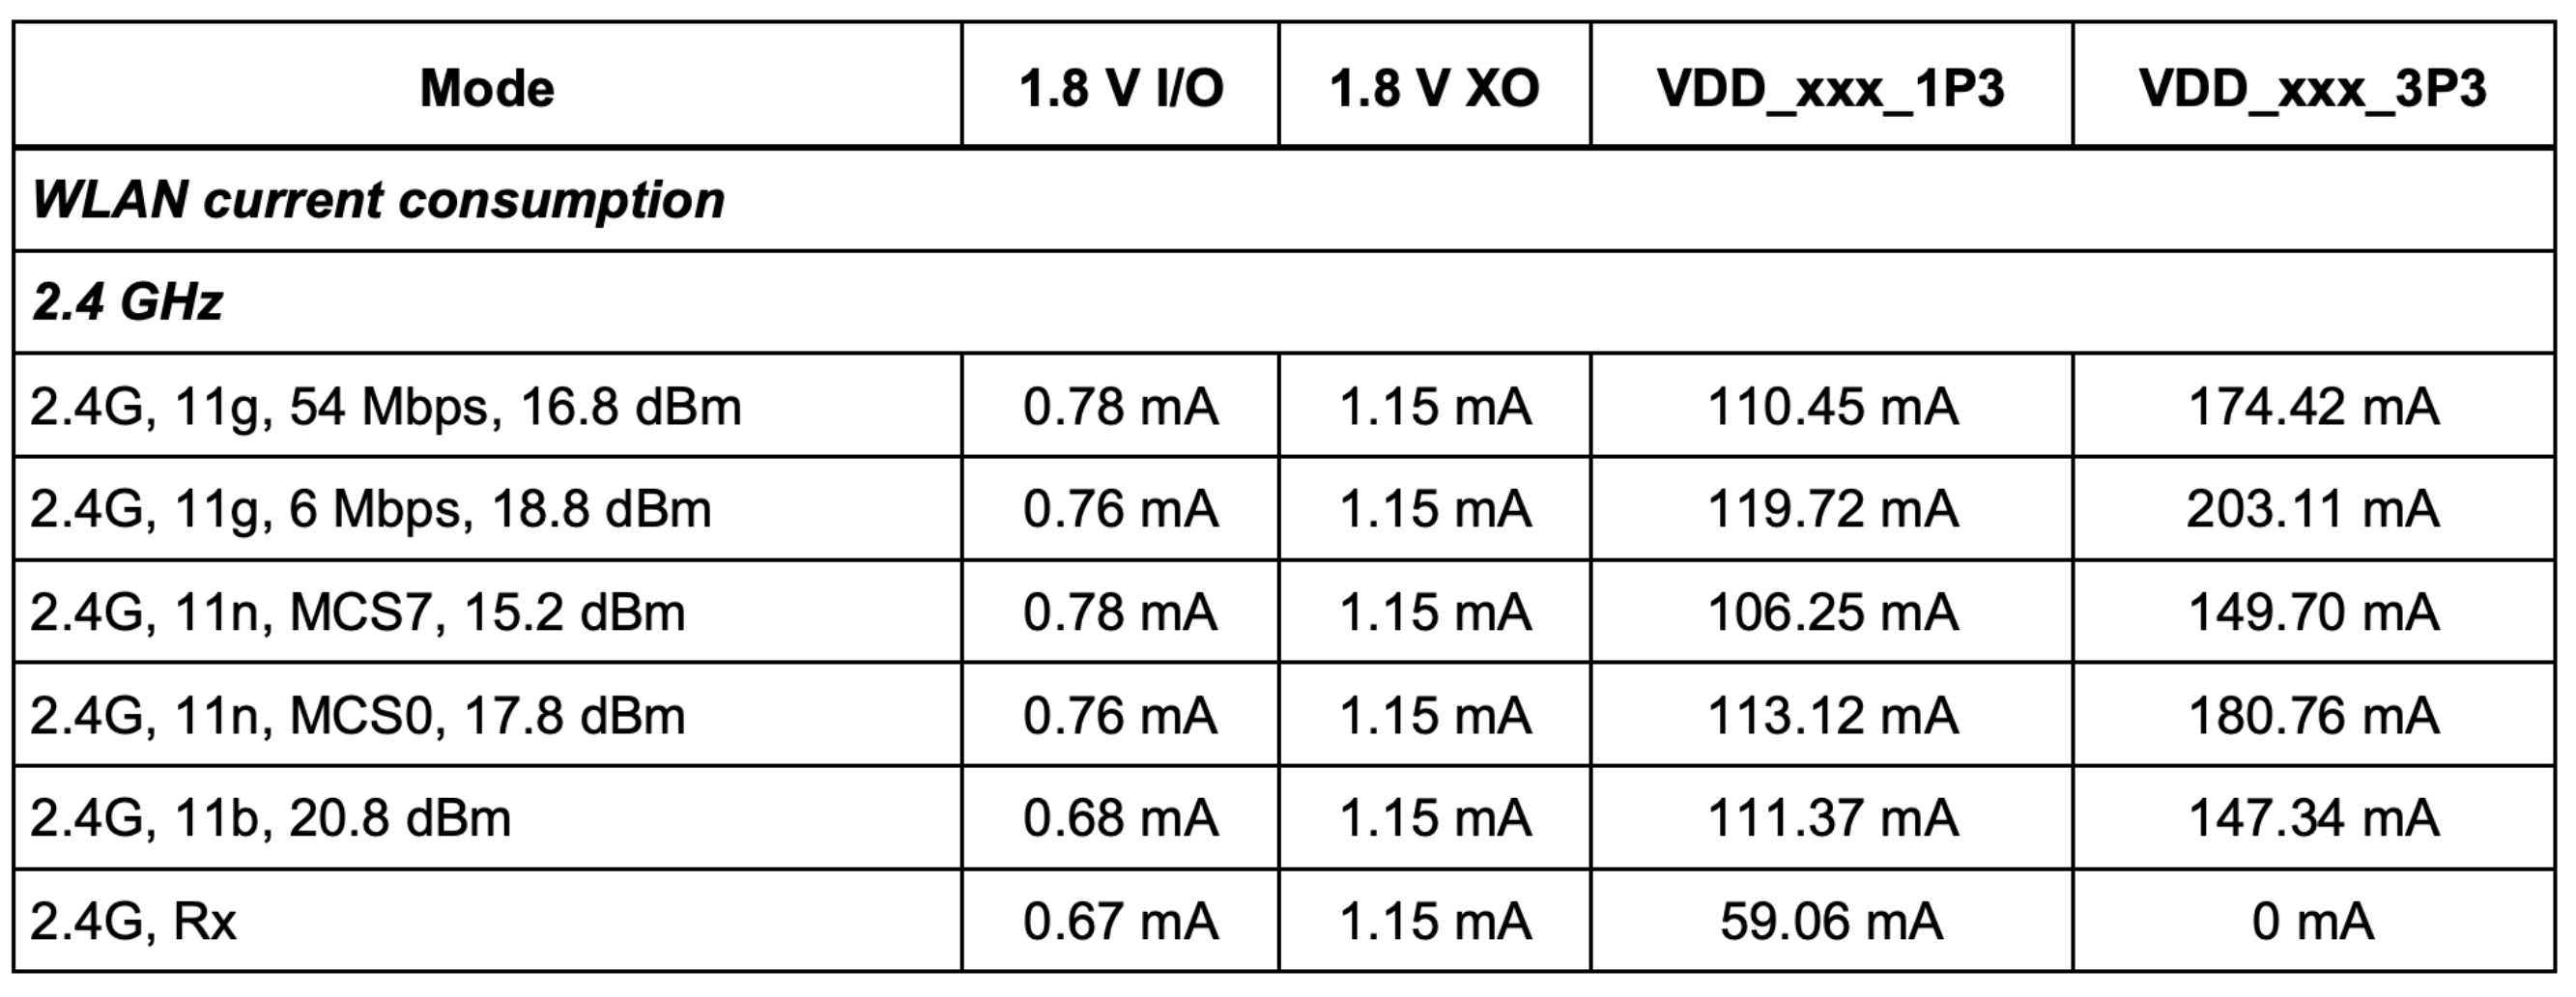
\includegraphics[scale=0.35]{Figs/wcndatasheet.png}    
    \end{center}
    \caption{Power Consumption values from WCN3620 Datasheet \cite{wcn3620}}
    \label{fig:wcn}
\end{figure}

Figure \ref{fig:wcn} shows the relevant power consumption information from the WCN3620 datasheet. Just like BCM43455, we can see there 
are two primary sources of voltage. One of them is $V_{xo}$ or $V_{cc}$ which is the voltage directly supplied by the battery/power source. 
The other one, $V_{I/O}$ is the voltage that the wifi adapter receives from the CPU indirectly. In order to compute the estimated power, 
we calculate the mean average sum of 2.4G, 11g and Rx values. We use 11g ones because the protocol standard being used is 802.11g. The other 
two voltage values are the operating voltages of the circuit and in this context, do not affect the calculations for the estimated 
power consumption. \\
To compute the power, we multiply current by voltage for each respective voltage and then take the average. This comes out to be 0.001737 Watts. 
In order to determine the optimal chunk size, we developed a simple script written in Java and deployed as an android app on the watch to 
run the experiments and extract a set of values. It uses the same communication API and protocols as the fall detection app. By utilizing the 
calculated power above, we were able to plot a graph between chunk size and energy consumption based off runtime information of the fall detection app.

\begin{figure}
    \begin{center}
        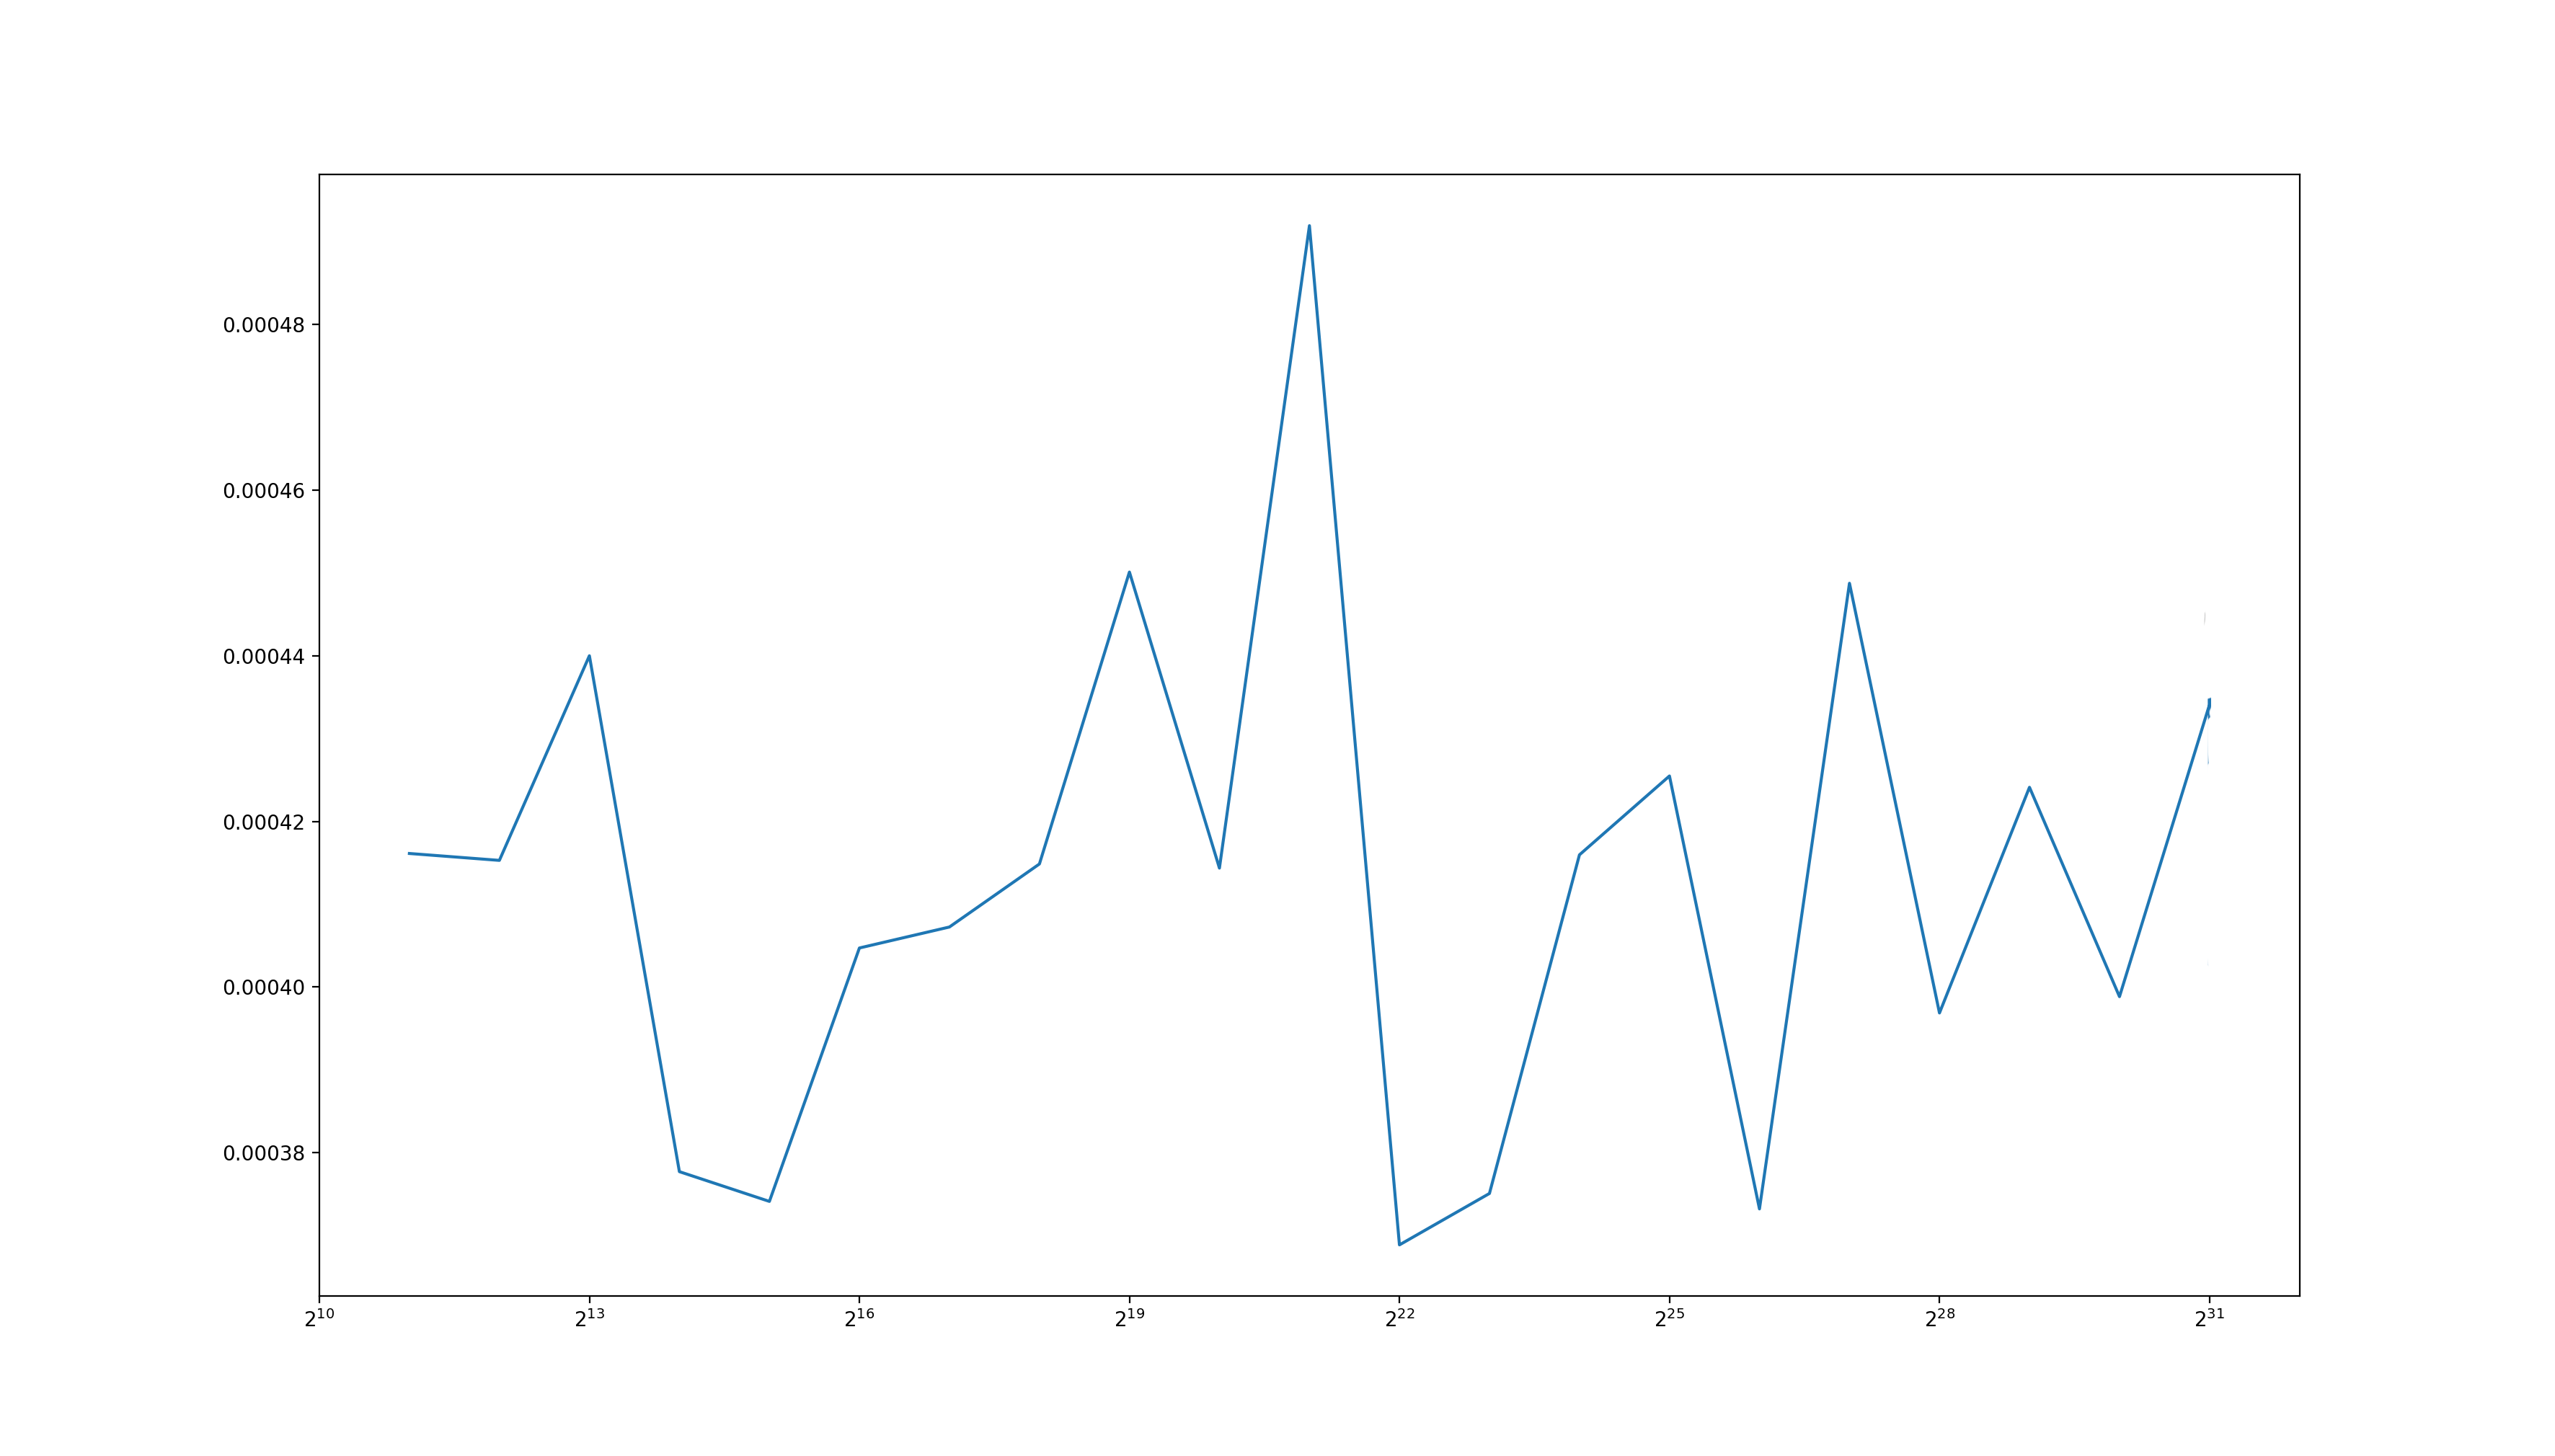
\includegraphics[scale=0.35]{Figs/energyandroid.png}    
    \end{center}
    \caption{EPB for different chunk sizes (Chunk Size (x-axis) and Energy in milliJ (y-axis)) - Huawei Watch}
    \label{fig:energyand}
\end{figure}

Figure \ref{fig:energyand} shows that the optimal chunk size for the Huawei Watch 2 is 4 Megabytes or $2^{22}$ bytes. Compare this with 
the default chunk size being used in the fall detection app of 340 Kilobytes which is about 12 times less than the optimal chunk size. 
However, this also required altering the communication interval of the app to one hour to have enough data accumulated to be able to send it.
This does not interfere with the actual detection functionality of the app. The overall reduction in wifi communication cost by using this 
chunk size is around 77.97\%. In this context, it is a significant improvement however, in terms of raw battery time saved, it is just around 
1.5 minutes. We would also like to mention here that the application failed to upload data to the server when we 
changed the chunk size to the optimal one. During our initial evaluation while running the Fall Detection application 
using Android Studio, it was successfully able to write data to the output stream that sends data to the server. Based off 
the energy estimation readings from that run, the improvement in battery time was around 1.5 minutes. However, when the 
application was run normally (without Android Studio), it was unable to upload the data to the server even though the 
data was being sent. There are a number of reasons for which this could be happening. First, the server may have an 
unintentional bottleneck that we are not aware of. Second, it may be possible that there is not sufficient 
space on the device to log an hour of data. Lastly, it could be something wrong with the implementation of the 
application \textemdash particularly how Couchbase is used to store the data in a local database. \\ 

Now let's talk about why the improvement is as small as 1.5 minutes. This is due to the fact that Huawei Watch 2 Sport in itself is a highly optimized smartwatch in terms of energy consumption. 
One of its selling point is its extended battery life due to lower energy consumption. However, our approach is still able to optimize the 
communication cost albeit only extending the battery life for a few minutes. One other factor that impacts this, is that the core functionality 
of the app itself is more focused on two things \textemdash displaying relevant information on the UI and constantly logging accelerometer data. 
Moreover, the constant logging is something that can not be altered in this case because the use case of the app is critical in nature. For 
instance, if we log data in sync with communication i.e. we only read and save sensor data 
when information needs to be transmitted to the server, it will definitely save more energy but it severely undermines the functionality of the app and 
ultimately fails to detect some critical fall cases at times when its not logging sensor data. This also shows why our work is more focused on 
communication cost only as this property is something that will rarely impact the use case of an app. \\
Moreover, the apps in our study are already somewhat optimized and well-written. Our approach would make even more significant impact if 
a developer wants to write an app from scratch and then matches the communication interval with the optimal chunk size i.e. when enough data is 
collected. In the next section, we will discuss a case study on comparing energy consumption of native apps, and apps in a container environment. 
